\section{سندباکس}


\begin{tikzpicture}
	\begin{axis}[
		% xmode=log,
		% ymode=log,
		legend style={at={(1,1)},anchor=north east
			,draw=none,fill=none,inner sep=2mm},
		xlabel=X, % \hertz requires SIunits
		ylabel=Y,
		title={Trajectory of the Satellite},
		% grid=both,
		% minor grid style={gray!25},
		% major grid style={gray!25},
		width=0.75\linewidth,
		enlarge y limits=0.15,
		no marks]
		\addplot[line width=1pt,solid,color=red] %
		table[x=x,y=y,col sep=comma]{../Code/Python/Environment/trajectory_latex.csv};
		\addlegendentry{Trajectory}
		\addplot[line width=1pt,dashed,color=black] %
		table[x=x,y=y,col sep=comma]{../Code/Python/TBP/PPO/DG/results/state.csv};
		\addlegendentry{PPO DG Trajectory}
	\end{axis}
\end{tikzpicture}

\begin{tikzpicture}
	\begin{axis}[
		% xmode=log,
		% ymode=log,
		legend style={at={(1,1)},anchor=north east
			,draw=none,fill=none,inner sep=2mm},
		xlabel=X, % \hertz requires SIunits
		ylabel=Y,
		title={Trajectory of the satellite},
		% grid=both,
		% minor grid style={gray!25},
		% major grid style={gray!25},
		width=0.75\linewidth,
		enlarge y limits=0.15,
		no marks]
		\addplot[line width=1pt,solid,color=blue] %
		table[x=x,y=y,col sep=comma]{../Code/Python/TBP/PPO/results/state.csv};
		\addlegendentry{Trajectory}
	\end{axis}
\end{tikzpicture}


\def\length{sqrt(1+(x-y)^2)}
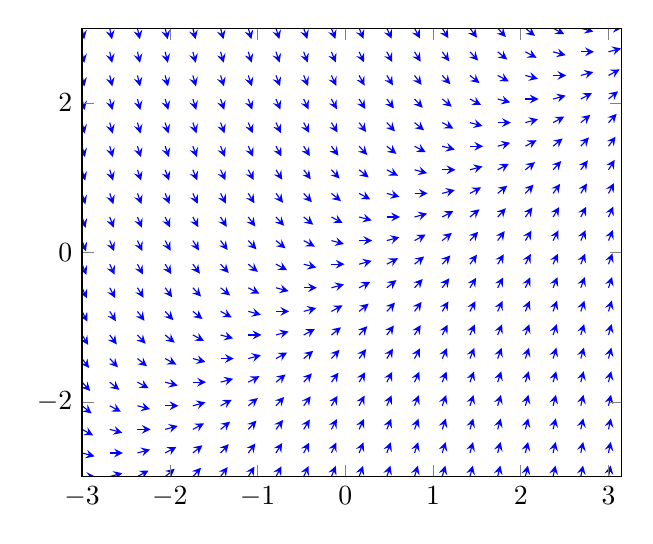
\begin{tikzpicture}
	\begin{axis}[domain=-3:3, view={0}{90}]
		\addplot3[blue, quiver={u={1/(\length)}, v={(x-y)/(\length)}, scale arrows=0.15}, -stealth,samples=20] {0};
	\end{axis}
\end{tikzpicture}


\begin{tikzpicture}
	\begin{axis}[
		% xmode=log,
		% ymode=log,
		legend style={at={(1,1)},anchor=north east
			,draw=none,fill=none,inner sep=2mm},
		xlabel=X, % \hertz requires SIunits
		ylabel=Y,
		title={Trajectory of the satellite},
		% grid=both,
		% minor grid style={gray!25},
		% major grid style={gray!25},
		width=0.75\linewidth,
		enlarge y limits=0.15,
		no marks]
		
		% Trajectory plot 1
		\addplot[line width=1pt,solid,color=blue] %
		table[x=x,y=y,col sep=comma]{../Code/Python/Environment/trajectory_latex.csv};
		\addlegendentry{Trajectory}
		
		% Trajectory plot 2 (PPO DG)
		\addplot[line width=1pt,solid,color=red] %
		table[x=ax,y=ay,col sep=comma]{../Code/Python/TBP/PPO/DG/results/action_state.csv};
		\addlegendentry{PPO DG Trajectory}
		
%		% Quiver plot: vector field
%		\addplot[quiver, -stealth, color=black, every axis plot/.append style={thick}] 
%		table[x=x,y=y,col sep=comma]{../Code/Python/TBP/PPO/DG/results/state.csv};
%		table[,u=ax,v=ay,col sep=comma] {../Code/Python/TBP/PPO/DG/results/action.csv}; % u and v for vector components
%		\addlegendentry{Vector Field}
		
	\end{axis}
\end{tikzpicture}


%\begin{tikzpicture}
%	\begin{axis}[
%		title={Trajectory of the Satellite},
%		xlabel=X, ylabel=Y,
%		width=0.75\linewidth,
%		enlarge y limits=0.15,
%		no marks
%		]
%		
%		% Define a custom function for the vector length
%		\def\length#1#2{sqrt(1 + (#1 - #2)^2)}  % Example length calculation function
%		
%		% Trajectory plot (positions from state.csv)
%		\addplot[line width=1pt, solid, color=blue] %
%		table[x=x, y=y, col sep=comma]{../Code/Python/TBP/PPO/DG/results/state.csv};
%		\addlegendentry{Trajectory}
%		
%		% Quiver plot: using x, y from state.csv and ax, ay from action.csv
%		\addplot[quiver, -stealth, color=black, every axis plot/.append style={thick}] 
%		table[x=x, y=y, u=ax, v=ay, col sep=comma] {../Code/Python/TBP/PPO/DG/results/action_state.csv}
%		\addlegendentry{Action Vectors}
%		
%	\end{axis}
%\end{tikzpicture}


%\begin{tikzpicture}
%	\begin{axis}[domain=-3:3, view={0}{90}]
%		
%		% Reading data from the CSV file and plotting the vectors
%		\addplot3[
%		blue, 
%%		quiver={
%%			u=1, % x-direction of the vector (ax from the table)
%%			v=1, % y-direction of the vector (ay from the table)
%%			scale arrows=0.15
%%		}, 
%		-stealth,
%		samples=20
%		] 
%		table[x=x, y=y] {../Code/Python/TBP/PPO/DG/results/action_state.csv}; % CSV file
%		
%	\end{axis}
%\end{tikzpicture}


